\documentclass[10pt,a4paper]{article}
\usepackage[utf8]{inputenc}
\usepackage[T1]{fontenc}
\usepackage{amsmath}
\usepackage{amssymb}
\usepackage{graphicx}
\usepackage{hyperref}
\usepackage{float}
\usepackage{subcaption}
\usepackage{geometry}
\geometry{a4paper, margin=1in}

\title{Exploring the Platonic Representation Hypothesis Beyond In-Distribution Data}
\author{Aryasomayajula Ram Bharadwaj\\
Independent Researcher\\
\texttt{ram.bharadwaj.arya@gmail.com}}
\date{20th Oct 2024}

\begin{document}

\maketitle

\begin{abstract}
The Platonic Representation Hypothesis (PRH) \cite{huh2024prh} suggests that models trained with different objectives and on various modalities can converge to a shared statistical understanding of reality. This paper explores whether PRH holds when models are exposed to out-of-distribution (OOD) data. We analyze the alignment of model representations using ImageNet-O, a dataset designed with OOD images, and compare these results with those from the original experiment where the evaluation data is within the pretraining data distribution and also with purely random data. Our findings indicate that PRH holds in OOD settings but not for random data, highlighting the importance of underlying structure in data for shared model representations.
\end{abstract}

\section{Introduction}
The PRH proposes that models converge toward a shared statistical representation of reality, regardless of training specifics such as dataset or training objectives. Previous evidence largely focused on available datasets which are in-distribution with respect to the training data of the models (e.g., Places365’s validation dataset). This hypothesis is extended here to include OOD scenarios using ImageNet-O and random noise data. The ImageNet-O dataset, as introduced in \cite{hendrycks2021nae}, contains images that lie outside the distribution of ImageNet, making it a valuable resource for testing generalization.

\section{Methodology}
To test PRH in OOD settings, we used various metrics for measuring model alignment, such as mutual k-NN and CKNN-A. The data was divided into three categories: (1) in-distribution data (ImageNet), (2) OOD data (ImageNet-O), and (3) random noise.

\section{Results}

\subsection{Vision-Vision Alignment on Places365’s Validation Dataset}
\begin{figure}[H]
    \centering
    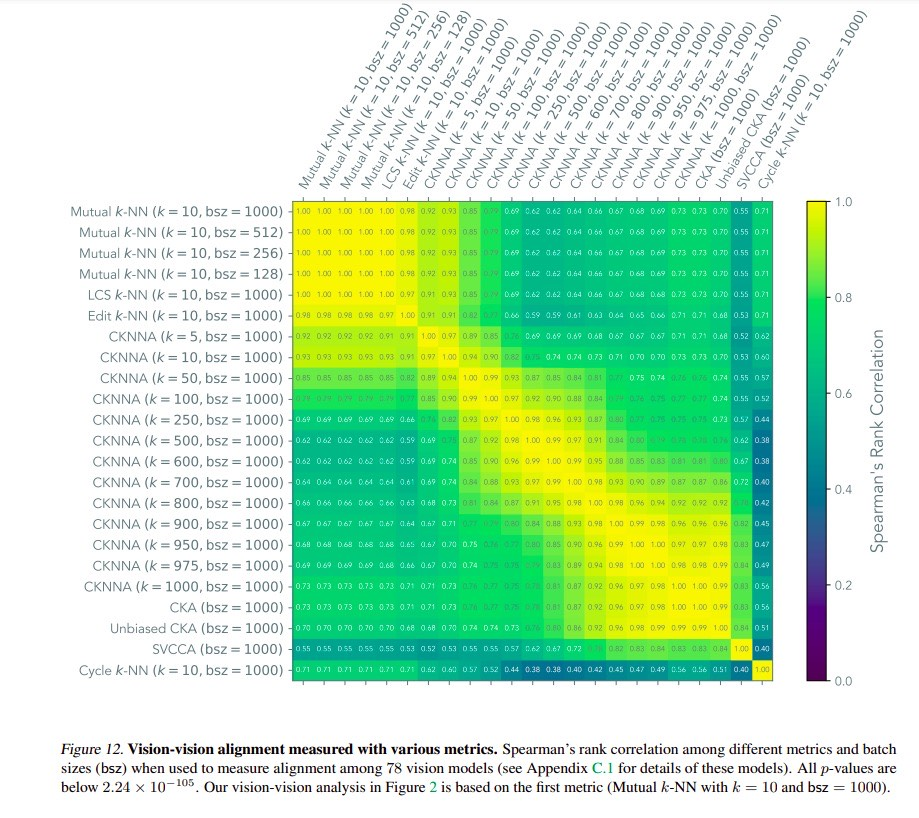
\includegraphics[width=\textwidth]{prh_correlation.jpg}
    \caption{Vision-vision alignment measured with various metrics. Spearman's rank correlation among different metrics and batch sizes when used to measure alignment among 78 vision models.}
    \label{fig:prh_correlation}
\end{figure}

\subsection{Vision-Vision Alignment on ImageNet-O}
\begin{figure}[H]
    \centering
    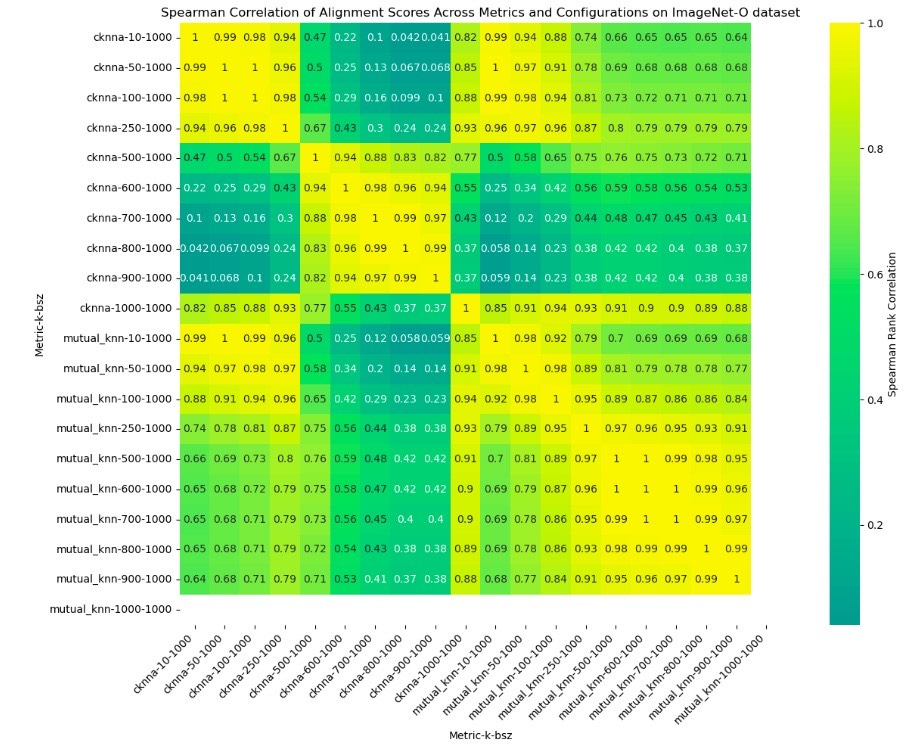
\includegraphics[width=\textwidth]{prh_correlation_ood.jpg}
    \caption{Spearman correlation of alignment scores across metrics and configurations on the ImageNet-O dataset.}
    \label{fig:prh_correlation_ood}
\end{figure}

\subsection{Vision-Vision Alignment on Random Data}
\begin{figure}[H]
    \centering
    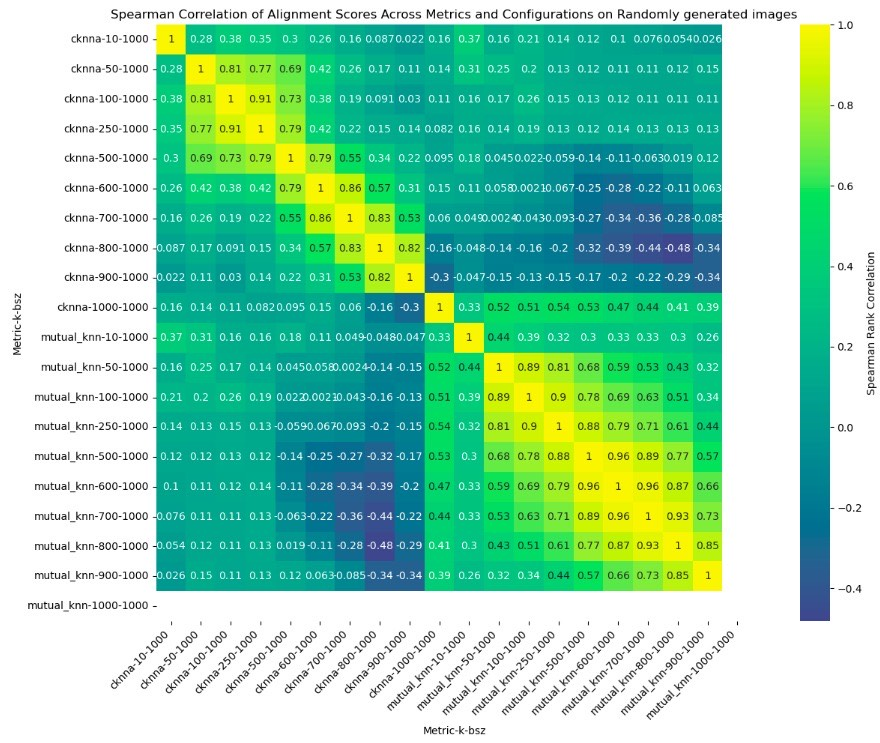
\includegraphics[width=\textwidth]{prh_correlation_random.jpg}
    \caption{Spearman correlation of alignment scores across metrics and configurations on randomly generated images.}
    \label{fig:prh_correlation_random}
\end{figure}

\section{Discussion}
The results suggest that the Platonic Representation Hypothesis (PRH) holds true even in out-of-distribution (OOD) settings, as demonstrated with the ImageNet-O dataset. Despite being exposed to outlier data, the models maintain high alignment in their representations, indicating that they might develop a shared underlying structure in their perception of reality, even when the training data distribution shifts. However, this alignment breaks down when models are exposed to purely random noise, revealing the limits of the PRH. This distinction is intriguing: on randomly generated data, models do not converge on a shared statistical understanding of reality. Yet, on OOD data like ImageNet-O, the models exhibit strong correlation in their representations, even though their predictions are consistently incorrect but made with high confidence. This suggests that, while the models fail on outlier data, their failure is systematic and predictable.

\section{Conclusion}
We have shown that PRH extends beyond in-distribution data, with models maintaining alignment even in OOD settings. However, the presence of underlying structure in data is crucial for such alignment. Future work should focus on developing better methods to test the generalizability of PRH, finding scenarios where the hypothesis might be falsified, and exploring cross-modality applications of PRH.

\vfill
The code used for the experiments and analysis in this paper is available on GitHub at \href{https://github.com/rokosbasilisk/prh-experiments}{https://github.com/rokosbasilisk/prh-experiments}.

\clearpage
\begin{thebibliography}{9}

\bibitem{huh2024prh}
Huh, M., Cheung, B., Wang, T., \& Isola, P. (2024). The Platonic Representation Hypothesis. \emph{International Conference on Machine Learning}.

\bibitem{hendrycks2021nae}
Hendrycks, D., Zhao, K., Basart, S., Steinhardt, J., \& Song, D. (2021). Natural Adversarial Examples. \emph{CVPR}. \href{https://arxiv.org/abs/2405.07987}{arXiv:2405.07987}.

\end{thebibliography}

\end{document}

